\documentclass{standalone}
\usepackage{tikz}
\usepackage{pgfplots}
\pgfplotsset{compat=1.18}

\begin{document}
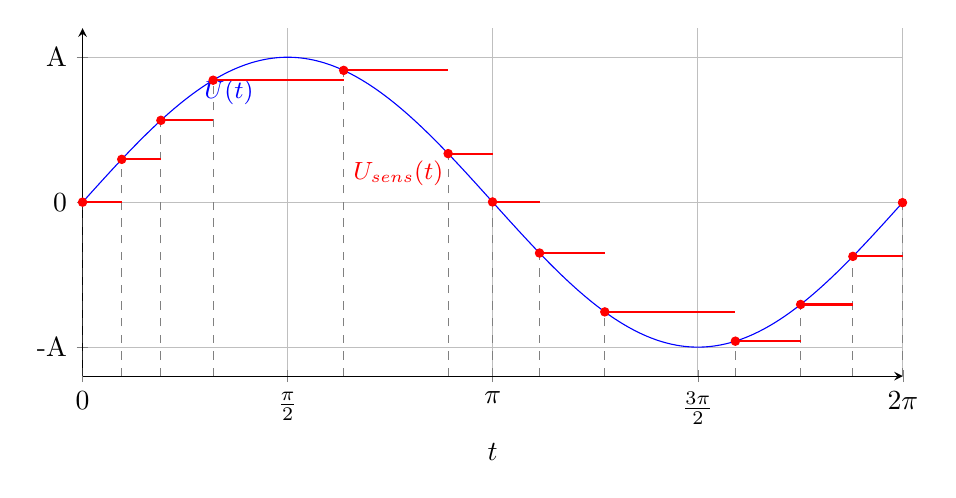
\begin{tikzpicture}
    \begin{axis}[
        width=12cm,
        height=6cm,
        xlabel={$t$},
        ylabel={},
        grid=major,
        xmin=0, xmax=6.28318,
        ymin=-1.2, ymax=1.2,
        xtick={0, 1.5708, 3.14159, 4.71239, 6.28318},
        xticklabels={$0$, $\frac{\pi}{2}$, $\pi$, $\frac{3\pi}{2}$, $2\pi$},
        ytick={-1, 0, 1},
        yticklabels={-A, 0, A},
        axis lines=left
    ]
        % Continuous signal
        \addplot[blue, domain=0:2*pi, samples=200, smooth] {sin(deg(x))} node[right, pos=0.15, font=\small] {$U(t)$};
        
        % Sample points (x-values)
        \pgfmathsetmacro{\xa}{0.0}
        \pgfmathsetmacro{\xb}{0.3}
        \pgfmathsetmacro{\xc}{0.6}
        \pgfmathsetmacro{\xd}{1.0}
        \pgfmathsetmacro{\xe}{2.0}
        \pgfmathsetmacro{\xf}{2.8}
        \pgfmathsetmacro{\xg}{3.14}
        \pgfmathsetmacro{\xh}{3.5}
        \pgfmathsetmacro{\xi}{4.0}
        \pgfmathsetmacro{\xj}{5.0}
        \pgfmathsetmacro{\xk}{5.5}
        \pgfmathsetmacro{\xl}{5.9}
        \pgfmathsetmacro{\xm}{6.28}
        
        % Draw vertical lines for sampling instants
        \foreach \xval in {\xa, \xb, \xc, \xd, \xe, \xf, \xg, \xh, \xi, \xj, \xk, \xl, \xm} {
            \addplot[gray, thin, dashed] coordinates {(\xval, -1.2) (\xval, {sin(deg(\xval))})};
        }

        % Draw the sampled signal (Zero-Order Hold)
        \draw[red, thick] (axis cs:\xa, {sin(deg(\xa))}) -- (axis cs:\xb, {sin(deg(\xa))});
        \draw[red, thick] (axis cs:\xb, {sin(deg(\xb))}) -- (axis cs:\xc, {sin(deg(\xb))});
        \draw[red, thick] (axis cs:\xc, {sin(deg(\xc))}) -- (axis cs:\xd, {sin(deg(\xc))});
        \draw[red, thick] (axis cs:\xd, {sin(deg(\xd))}) -- (axis cs:\xe, {sin(deg(\xd))});
        \draw[red, thick] (axis cs:\xe, {sin(deg(\xe))}) -- (axis cs:\xf, {sin(deg(\xe))});
        \draw[red, thick] (axis cs:\xf, {sin(deg(\xf))}) -- (axis cs:\xg, {sin(deg(\xf))});
        \draw[red, thick] (axis cs:\xg, {sin(deg(\xg))}) -- (axis cs:\xh, {sin(deg(\xg))});
        \draw[red, thick] (axis cs:\xh, {sin(deg(\xh))}) -- (axis cs:\xi, {sin(deg(\xh))});
        \draw[red, thick] (axis cs:\xi, {sin(deg(\xi))}) -- (axis cs:\xj, {sin(deg(\xi))});
        \draw[red, thick] (axis cs:\xj, {sin(deg(\xj))}) -- (axis cs:\xk, {sin(deg(\xj))});
        \draw[red, thick] (axis cs:\xk, {sin(deg(\xk))}) -- (axis cs:\xl, {sin(deg(\xk))});
        \draw[red, thick] (axis cs:\xl, {sin(deg(\xl))}) -- (axis cs:\xm, {sin(deg(\xl))});
        
        % Draw markers at sample points on the blue curve
        \foreach \xval in {\xa, \xb, \xc, \xd, \xe, \xf, \xg, \xh, \xi, \xj, \xk, \xl, \xm} {
            \addplot[only marks, mark=*, mark size=1.5pt, red] coordinates {(\xval, {sin(deg(\xval))})};
        }
        
        \node[right, color=red, font=\small] at (axis cs:2.0, 0.2) {$U_{sens}(t)$};

    \end{axis}
\end{tikzpicture}
\end{document}
